\documentclass[a4paper,notitlepage]{article}
\usepackage[utf8]{inputenc}
\usepackage[T1]{fontenc}
\usepackage[english]{babel}
\usepackage{amsfonts,amsmath,amssymb,amsthm,graphicx}
\usepackage[pdftex,hidelinks]{hyperref}
\usepackage{tikz}
\usetikzlibrary{arrows,shapes,automata,petri}

\usepackage{enumerate}
\usepackage{verbatim}
\usepackage{csquotes}
\usepackage{cite}
\usepackage{algorithm}
%\usepackage{algorithmic}
\usepackage{algpseudocode}

\newcommand{\HIDE}[1]{}
\newtheorem{thm}{Theorem}

\title{Distributed Systems Assignment 2\\ \large{Part 2}}
\author{John L\r{a}ng, Suravi Roy}

\begin{document}

    \maketitle
   	\begin{enumerate}[1.]
   		\item
   			\begin{enumerate}[1)]
   			\item
	   			The Petri net given in this question has only four reachable markings,
   				$M_1$, $M_2$, $M_3$, and $M_4$, as demonstrated in Figures \ref{fig1} and
   				\ref{fig2}. Asterisks (`*') denote enabled transitions. In the initial
   				marking, $M_1$, only the transition $t_2$ may fire, which leads the Petri
	   			net into marking $M_2$. In marking $M_2$, only $t_1$ may fire, so the
   				Petri net transitions into marking $M_3$. In marking $M_3$, the only
   				enabled transition is $t_3$, which transforms the Petri net into marking
   				$M_4$. After marking $M_4$, the Petri net transitions back into marking
	   			$M_1$, as $t_1$ is the only enabled transition.
   			
   				Since in every one of these four markings, there is only one enabled
   				transition, the Petri net is deterministic and the sequence of markings
   				repeats infinitely
	   			\begin{align}
   				    M_1 \to M_2 \to M_3 \to M_4 \to M_1 \to ...
   				\end{align}
   				According to the English Wikipedia article on Petri nets, a Petri net is
	   			$L_k$-live if and only if all of its transitions are $L_k$ live. In this
   				case, the definition of $L_3$-liveness applies to the Petri net under
   				investigation, as there is the infinite firing sequence (1) in which
   				every transition fires infinitely often.
	    		\begin{figure}
	    			\centering
   					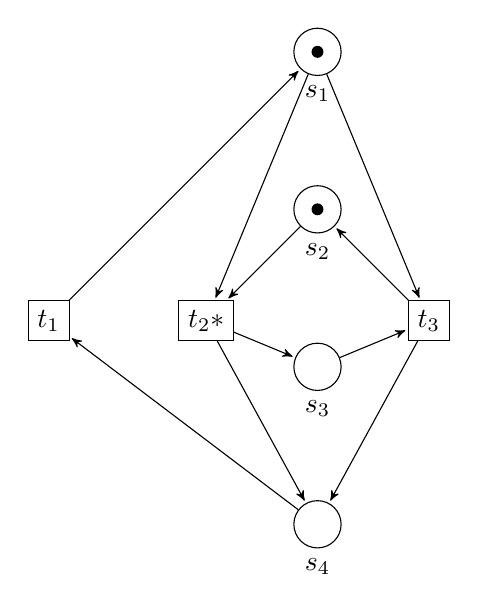
\begin{tikzpicture}[node distance=2cm,>=stealth',bend angle=45,auto]

		  				\tikzstyle{place}=[circle,draw=black,minimum size=6mm]
						\tikzstyle{transition}=[rectangle,draw=black,minimum size=4mm]
	    				\node [place,tokens=1,label=below:$s_1$] (s1) {};
   						\node [place,tokens=1,label=below:$s_2$] (s2) [below of=s1] {};
   						\node [place,label=below:$s_3$] (s3) [below of=s2]  {};
		    			\node [place,label=below:$s_4$] (s4) [below of=s3]  {};
	   					\node [transition] (t2) [below left of=s2] {$t_2*$}
   							edge [pre]  (s1)
	      					edge [pre]  (s2)
   							edge [post] (s3)
   							edge [post] (s4);

	    				\node [transition] (t1) [left of=t2] {$t_1$}
  							edge [pre]  (s4)
	  						edge [post] (s1);

	    				\node [transition] (t3) [below right of=s2] {$t_3$}
  							edge [pre]  (s1)
  							edge [pre]  (s3)
	    	 				edge [post] (s2)
  							edge [post] (s4);
					\end{tikzpicture}
					\hspace{1cm}
	    			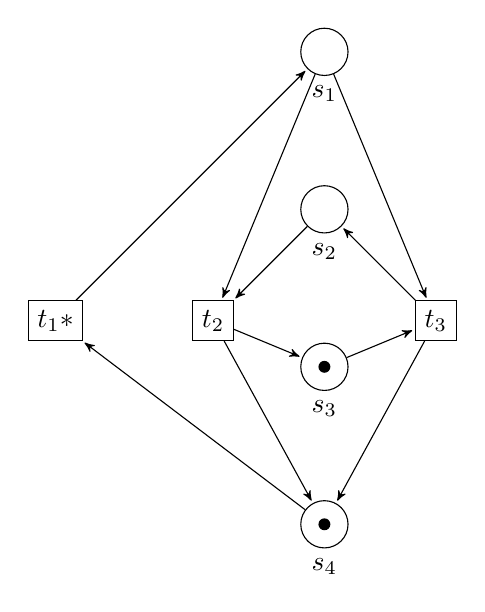
\begin{tikzpicture}[node distance=2cm,>=stealth',bend angle=45,auto]

	  					\tikzstyle{place}=[circle,draw=black,minimum size=6mm]
  						\tikzstyle{transition}=[rectangle,draw=black,minimum size=4mm]

	    				\node [place,label=below:$s_1$] (s1) {};
    					\node [place,label=below:$s_2$] (s2) [below of=s1] {};
		    			\node [place,tokens=1,label=below:$s_3$] (s3) [below of=s2] {};
    					\node [place,tokens=1,label=below:$s_4$] (s4) [below of=s3] {};

    					\node [transition] (t2) [below left of=s2] {$t_2$}
			      			edge [pre]  (s1)
      						edge [pre]  (s2)
	      					edge [post] (s3)
		      				edge [post] (s4);

    					\node [transition] (t1) [left of=t2] {$t_1*$}
      						edge [pre]  (s4)
			      			edge [post] (s1);

    					\node [transition] (t3) [below right of=s2] {$t_3$}
	      					edge [pre]  (s1)
		      				edge [pre]  (s3)
      						edge [post] (s2)
      						edge [post] (s4);
					\end{tikzpicture}
    				\caption{The fist two markings ($M_1$ on the left and $M_2$ on the right).}
			    	\label{fig1}
			    \end{figure}
    			\begin{figure}
			    	\centering
    				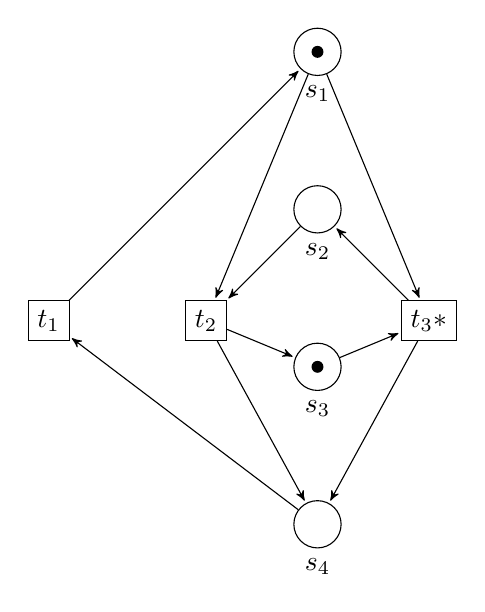
\begin{tikzpicture}[node distance=2cm,>=stealth',bend angle=45,auto]

	  					\tikzstyle{place}=[circle,draw=black,minimum size=6mm]
		  				\tikzstyle{transition}=[rectangle,draw=black,minimum size=4mm]

    					\node [place,tokens=1,label=below:$s_1$] (s1) {};
    					\node [place,label=below:$s_2$] (s2) [below of=s1] {};
			    		\node [place,tokens=1,label=below:$s_3$] (s3) [below of=s2] {};
    					\node [place,label=below:$s_4$] (s4) [below of=s3] {};

	    				\node [transition] (t2) [below left of=s2] {$t_2$}
		      				edge [pre]  (s1)
      						edge [pre]  (s2)
      						edge [post] (s3)
		    	  			edge [post] (s4);

    					\node [transition] (t1) [left of=t2] {$t_1$}
    	  					edge [pre]  (s4)
			      			edge [post] (s1);

    					\node [transition] (t3) [below right of=s2] {$t_3*$}
      						edge [pre]  (s1)
		    	  			edge [pre]  (s3)
      						edge [post] (s2)
    	  					edge [post] (s4);
					\end{tikzpicture}
					\hspace{1cm}
		    		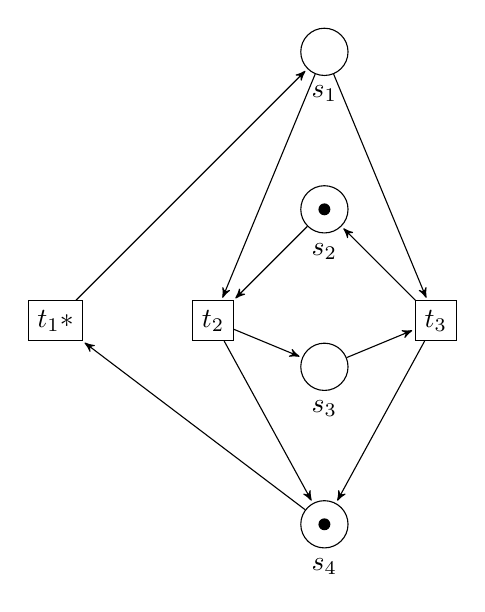
\begin{tikzpicture}[node distance=2cm,>=stealth',bend angle=45,auto]

  						\tikzstyle{place}=[circle,draw=black,minimum size=6mm]
  						\tikzstyle{transition}=[rectangle,draw=black,minimum size=4mm]

			    		\node [place,label=below:$s_1$] (s1) {};
    					\node [place,tokens=1,label=below:$s_2$] (s2) [below of=s1] {};
	    				\node [place,label=below:$s_3$] (s3) [below of=s2] {};
		    			\node [place,tokens=1,label=below:$s_4$] (s4) [below of=s3] {};

    					\node [transition] (t2) [below left of=s2] {$t_2$}
      						edge [pre]  (s1)
			      			edge [pre]  (s2)
    	  					edge [post] (s3)
	      					edge [post] (s4);

			    		\node [transition] (t1) [left of=t2] {$t_1*$}
    	  					edge [pre]  (s4)
	      					edge [post] (s1);

		    			\node [transition] (t3) [below right of=s2] {$t_3$}
      						edge [pre]  (s1)
    	  					edge [pre]  (s3)
			      			edge [post] (s2)
      						edge [post] (s4);
					\end{tikzpicture}
    				\caption{The next two markings ($M_3$ on the left and $M_4$ on the right).}
		    		\label{fig2}
    			\end{figure}
    		\item
    			We produced a reachability graph of the second Petri net in this exercise
    			by using WoPed. The result can be found in the bitmap image
    			\texttt{Question2.png}. As the reachability graph shows, all of the 17
    			markings reachable from the initial marking belong to the same strongly
    			connected graph (component). This Petri net is at least $L_2$-live,
    			because every transition can be fired arbitrarily often, as the
    			reachability graph shows.
    		
    			Consider the vertex ``\texttt{( p1 p3 p6...}``. All cycles in the
    			reachability graph pass through it. The only incoming edge to this
    			vertex is labeled $t_3$, which means that all cycles have to contain
    			$t_3$, making $t_3$ satisfy $L_3$-liveness. This vertex has two outgoing
    			edges labeled $t_1$ and $t_4$. The destination of the latter has only one
    			outgoing edge, labeled as $t_1$. Thus, the transition $t_1$ also satisfies
    			$L_3$-liveness. A similar argument starting from the vertex
    			``\texttt{( p1 p3 p6...}`` on the bottom-right side of the reachability
    			graph shows that $t_5$ is also $L_3$ live. It can be reasoned further,
    			that $t_2$ and $t_4$ are also $L_3$-live, by considering one step farther
    			in the reachability graph.
    		\item
    			We also produced a reachability graph for the third Petri net using
    			WoPeD, and saved it to the bitmap image \texttt{Question3.png}. It is
    			more complex than in the previous case, but it can be seen that for
    			instance, the edges 1 and 106 both represent the marking
    			\begin{align*}
    				p_1, p_2, p_5, p_6, p_9, p_{10}
				\end{align*}    			 
				and the path between these edges is non-trivial. This means that the
				path represents a cycle in a firing sequence, so the second Petri net is
				live at least in the sense that there exists an infinite firing sequence,
				namely the one that repeats this cycle forever.
    		\end{enumerate}
    	\item
    		\begin{enumerate}[1)]
    			\item
    				From the Figures 1 and 2 it shows that all of the places in the first
    				Petri net are 1-bounded.
				\item    				
    				Because the reachability graph of the second Petri net is finite, it
    				follows that every firing sequence keeps cycling through a finite
    				number of markings. For every place, the maximum bound of tokens can
    				be determined from the reachability graph, by checking which of the
    				markings place the largest number of tokens in that place. In this
    				case, all places happen to be 1-bounded.
    			\item
    				The transitions of the third Petri net can be represented as the
    				following $12 \times 7$ matrix:
    				\begin{equation*}
    					\mathbf{C} =
    						\left( \begin{matrix}
  								 1 & -1 & -1 &  0 &  0 &  0 &  0 \\
  								 0 & -1 &  1 &  0 &  0 &  0 &  0 \\
  								 0 &  1 & -1 &  0 &  0 &  0 &  0 \\
  								-1 &  1 &  1 &  0 &  0 &  0 &  0 \\
  								 0 &  0 &  1 & -1 & -1 &  0 &  0 \\
  								 0 &  0 &  0 & -1 &  1 &  0 &  0 \\
  								 0 &  0 &  0 &  1 & -1 &  0 &  0 \\
  								 0 &  0 & -1 &  1 &  1 &  0 &  0 \\
  								 0 &  0 &  0 &  0 &  1 & -1 & -1 \\
  								 0 &  0 &  0 &  0 &  0 & -1 &  1 \\
  								 0 &  0 &  0 &  0 &  0 &  1 & -1 \\
  								 0 &  0 &  0 &  0 & -1 &  1 &  1 \\
 							\end{matrix} \right)
    				\end{equation*}
    				Since all columns sum to zero, it holds that
    				\begin{equation*}
    				    (1,1,1,1,1,1,1,1,1,1,1,1) \times \mathbf{C} = \mathbf{0},
    				\end{equation*}
    				regardless of the initial marking. It follows by a known result\footnote{
    				\url{http://wwwis.win.tue.nl/~wvdaalst/old/courses/BIScourse/BIS-12-structural-subclasses.pdf},
    				p. 35}
    				that the third Petri net is bounded.
    		\end{enumerate}
   		\item
    		\begin{enumerate}[1)]
    			\item
    				The marking, in which all odd-numbered places have tokens, is $M_3$.
    				The shortest firing sequence that reaches $M_3$ from the initial marking
    				$M_1$ is
    				\begin{align*}
    				    M_1 \to M_2 \to M_3.
    				\end{align*}
   
    			\item
    				For the second petri net, the marking in which all the odd-numbered
    				places have a token is the one where the tokens are in places $p_1$,
    				$p_3$, $p_5$, and $p_7$. A shortest firing sequence to this marking has
    				to remove the token from $s_6$. The only transition that can do this is
    				$t_4$. Similarly, the only transition that can remove the token from
    				$s_2$ is $t_2$. These two transitions are independent of each other,
    				so it doesn't matter which one fires first in a shortest firing
    				sequence. After $t_2$, $t_1$ needs to fire and the place $s_8$ has to
    				have a token in order to enable $t_3$. After $t_3$ has fired, the part
    				of the Petri net to the right of $t_3$ has the correct marking. At this
    				point, it remains to remove tokens from $s_2$ and $s_4$ and move tokens
    				to places $s_1$ and $s_3$. This can be accomplished by firing the
    				transitions $t_1$, $t_2$, and $t_1$ again.
    				
    				The three firing sequence fitting the description above, described in
    				terms of transitions, are
    				\begin{align*}
    				    &t_2, t_1, t_4, t_3, t_1, t_2, t_1; \\
    				    &t_2, t_4, t_1, t_3, t_1, t_2, t_1;\text{ and }\\
    				    &t_4, t_2, t_4, t_3, t_1, t_2, t_1.
    				\end{align*}
    				Therefore, the length of the shortest firing sequences leading to the
    				marking where all odd-numubered places have a token is 7.
    				
    			\item
    				Following the approach described above, for the shortest firing
    				sequence leading to the marking that puts tokens in odd-numbered places
    				starts with any permutation of $t_2$, $t_4$, and $t_6$ followed by the
    				firing sequence
    				\begin{align*}
    				    t_1, t_3, t_5, t_1, t_2, t_1, t_3, t_4, t_1, t_2, t_1, t_3, t_1, t_2, t_1.
    				\end{align*}
    				All of these six shortest paths have length 18.
    		\end{enumerate}
    	\item
   			To mark the odd-numbered places in the $n$th member, the following
   			algorithm can be used:
   			\begin{itemize}
   				\item
   					The two places with the highest indices have to be marked in the $n$th 
   					member by firing the transition $t_{2n}$.
   				\item
   					Also, the transitions $t_{2n-2}$ and $t_{2n-3}$ must be fired.
   				\item
   					After performing the previous two steps, firing the transition
   					$t_{2n-1}$ marks the odd-numbered places in the $n$th member.
			\end{itemize}   			
			There are two possible firing sequences that accomplish
   			the desired marking:
   			\begin{align*}
   				t_{2n}, t_{2n-2}, t_{2n-3}, t_{2n-1} \\
   				t_{2n-2}, t_{2n-3}, t_{2n}, t_{2n-1}
   			\end{align*}
   			Repeating this algorithm for all members in decreasing order produces a
   			shortest firing sequence to a marking with tokens in all odd-numbered
   			places.
   	\end{enumerate}
\end{document}
